\documentclass[12pt, a4paper]{ujreport} % a4jでもOKっぽい

%% ----- packages ----- %%
% --- 図表 --- %
\usepackage{plautopatch}
\usepackage[dvipdfmx]{graphicx, xcolor, pict2e} % geometory: 余白設定 graphicx: 画像挿入 xcolor: 文字の色付け pict2e: 図が描ける
\usepackage{here} % 図の配置を指定できる
\usepackage{float} % here と同じらしい
\usepackage{longtable} % 表
\usepackage{colortbl} % 表に色を付ける
\usepackage{tabularx} % 表組みの設定
\usepackage{enumerate} % 番号付き箇条書き
\usepackage{lscape} % 図表回転
\usepackage{multirow} % 表のセルに連続して同じ値を書くときにまとめて書ける(行)
\usepackage{diagbox} % 表ヘッダ作成
\usepackage{multicol} % 表のセルに連続して同じ値を書くときにまとめて書ける(列)
\usepackage{wrapfig} % 図と文章を並べて書ける
\usepackage{hhline}
% \usepackage{graphicx}

% --- 文字 --- %
\usepackage{bm} % 太字の斜体
\usepackage{underscore} % アンダーバー"_"を表示できる
\usepackage{plext} % 縦書きを横書きで書ける
\usepackage{fancyhdr} % ヘッダとフッタを編集できる
\usepackage{ulem} % 下線が引ける
\usepackage{cite} % 参考文献リスト"bibitem"の参照
\usepackage{times} % フォント "times" に指定
\usepackage{mathptmx} % 数式も含めてフォント "times" に指定
\usepackage{amsmath,amssymb,amsfonts} % 数式をきれいに書ける。amsfontsはフォントを指定しているが、mathptmxでフォント指定されているため、機能していない。
\usepackage{algorithmic} % アルゴリズム(疑似コード)を書ける
\usepackage{textcomp} % 特殊文字を書ける
\usepackage{comment} % コメントアウト
\usepackage{url} % url挿入
%\usepackage[ipaex]{pxchfon} %文書内の和文フォントの指定(ipaexフォントが指定されている, 無くても大丈夫そう)
%\usepackage[uplatex, deluxe]{otf}

%% --- ページ設定 --- %%
% \usepackage[top=30truemm,bottom=30truemm,left=30truemm,right=20truemm]{geometry} % 余白設定

% (すぐ上の行を使わないとき用)
\makeatletter
% \setlength{\voffset}{0.5truecm} % old 上余白 (1)
% \setlength{\oddsidemargin}{7.0truemm} % old 左余白 (3): 25.4mm + 7.0mm = 32.4mm
\setlength{\oddsidemargin}{4.6truemm} % 左余白: 25.4mm + 4.6mm = 30mm, 13pt
% \setlength{\evensidemargin}{-5.5truemm} % old 偶数頁左余白 (3): 25.4 - 5.5mm = 19.9mm, jreportなので不要?
% \setlength{\topmargin}{-1truecm} % old (4)
\setlength{\topmargin}{-23pt} % -12pt+(-11pt) = -23pt, 8.1mm (4)
% \setlength{\headsep}{2truecm} % old 上余白 (6)
\setlength{\headsep}{25pt} % 8.81mm, 12pt+14pt=25pt (6), 上余白30mmになるように設定した
% \setlength{\textheight}{22truecm} % old (7)
\setlength{\textheight}{672pt} % 845pt-85pt*2, 237truemm (7), 下余白30mmになるように設定した
% \setlength{\textwidth}{15truecm} % old (8)
\setlength{\textwidth}{441pt} % (8) 155truemm, 右余白25mmになるように設定した
% \setlength{\footskip}{25truemm} % old (11)
\setlength{\footskip}{30pt} % 10.5pt+19.5pt=30pt, 10.6mm(11), ページ数の位置
% 1pt = 0.35mm
\makeatother


%% ----- main ----- %%
\begin{document}

\pagenumbering{roman}
\title{
タイトル未定\\
untitled
}
\author{
指導教員: 小松川 浩 \\
公立千歳科学技術大学 理工学部 \\
理工学専攻 博士前期課程2年 \\
小松川・山川・深町研究室 \\
令和5年度 \\
m2220180 新井田 響}
\date{\today}
\maketitle

\tableofcontents
\thispagestyle{empty}

\chapter{序論\label{c1}}
\pagenumbering{arabic}

\section{背景}
現在,レポートや論文の書き方をはじめとする文章作成技法に関する講義が開講され,様々な教育機関において文章作成能力の向上が求められている.一方で,文章作成技法に関する講義の指導方法は各教育機関や教員によって異なり,模範となる指導方法は確立されていない.これは大学についても同様である.
レポートや論文は,学術的文章に適した表現で記述することが求められる.しかし,学術表現に従ったレポートを作成できない学生が多く存在し,特に,文章中に話しことばが混在することが問題視されている.これらの課題に対し,本研究チームは,話しことばの情報を集約割いたデータベースを活用し,話しことばカテゴリに基づく添削を行う大学初年次向け文章添削システム「話しことばチェッカー」に関する研究を行ってきた.

ある表現が話しことばであるか書きことばであるかが採点者によって解釈が分かれる可能性のある曖昧な表現が存在し、文章作成において一貫した指導が難しいとされている。その要因として、あいまいな表現が,話しことばであるか書きことばであるかが文脈の中でどのように用いられているかによって決まる表現が存在することが挙げられる。一方で本システムでは、ルールベースのアルゴリズムに基づく話しことば検出を行うため、正しい検出結果を示すことができないという課題がある。以上のような文脈によって話しことばとも書きことばともとれる表現が存在することがわかっており、本研究チームではこの表現を「グレーゾーン」と定義している。

近年発達してきた機械学習の手法を用いることによって文章内の単語の位置関係以外にも,文脈を考慮した単語の位置関係の把握も行えるようになってきた.また,インターネットの発展とともに,文章や画像のデータセットを無償で利用できることも可能になってきている.先行研究では,グレーゾーンを含む文章が主観的であれば,そのグレーゾーンは話しことば,客観的であれば書きことばに分類できるという仮定のもと,インターネットから収集したグレーゾーンを含む文章を学習させ,グレーゾーンの判別が可能な機械学習モデルの構築を試みた.

しかし,学習データや検証データの確保については,手作業による事例収集やラベル付けについても,専門家が個々のデータを見て判断する必要があるなどといった問題がある.すべてのグレーゾーンの判別が可能な機械学習モデルを構築するために各々のグレーゾーン用のデータセットを作成することは現実的ではない.

\section{目的}


\section{構成}
本論文の構成について述べる.
 % 背景目的
\chapter{第2章予定地\label{c2}}

\section{先行研究 \label{c2s1}}
「話しことばチェッカーの開発と実証評価」は本研究チームの山下による研究である.レポートに含まれる話しことばの個数を,話しことばチェッカーによる判定を受ける前後でどのように変化したかについて述べられている.今後の課題として,システムの誤検出およびパターンマッチでは判断しきれない表現への対応が挙げられており,機械学習を活用した文脈判断による話しことば検出の必要があると述べられている.パターンマッチでは判断しきれない曖昧な表現の例として「~てしまう」が挙げられ,その表現が出現する文章の主語が一人称であれば主観的,三人称であれば客観的となり,機械学習を用いることでそれぞれ話しことば,書きことばに分類できる可能性が示唆されている.

「学生のレポートにおける話し言葉とその出現傾向」は本研究チームの山下による研究である.レポートの書き方に関する書籍で取り扱われる話しことばについてまとめ,「学術文章作法I」で提出された学生のレポートから抽出した話しことばについて分析している.ある表現について,話しことばか書きことばかの判断が添削者により異なる表現が存在することや,話しことばをどのように書きことばに書き改めるべきかの判断が難しい事例が存在することなどが示されている.具体例として,「~から」「~ので」について,それぞれを「~ために」に書き改めるよう指示している場合や,「~から」を「~ので」への置き換えを許容する場合が存在する.本研究チームでは,文章に含まれる話しことばを検出する Web システムである話しことばチェッカーの研究および開発を行っているが,このような曖昧な表現について柔軟に対応ができないという課題がある. % 先行研究位置づけ
\chapter{第3章予定地\label{c3}}

% 話しことばチェッカー関連

\section{話しことばの定義 \label{c3s1}}
本研究チームにおける「話しことば」の定義は,特に大学初年次の学生が自らレポート推敲が行えることが望ましい非学術的な表現と定義されている.ただし,本研究チームにおいての話しことばは,口語的意味合いによる話し言葉ではなく,レポートや論文などの文章に現れる「書かれた話し言葉」を指す.

\section{話しことばカテゴリ \label{c3s2}}
これまでの研究により,話しことばには,単語そのものが話しことばである表現や,単語の位置関係,例えばある単語の直前にある単語との組み合わせによって話しことばと判断される表現が存在することがわかっている.これらの表現に対し,本研究チームでは「話しことばカテゴリ」と定義している.カテゴリは,表3.1に示すように,前述のような単語の位置関係や品詞などに応じて5つに分類される.

\begin{table}[H]
\centering
\caption{話しことばカテゴリ}
\begin{tabular}{|c|l|l|l|}
\hline
\multicolumn{1}{|c|}{番号} & \multicolumn{1}{c|}{名称} & \multicolumn{1}{c|}{説明} & \multicolumn{1}{c|}{例} \\ \hline
1 & INDEPENDENCE & 対象の単語がある           & \begin{tabular}[c]{@{}l@{}}当たり前、\\あんまり\end{tabular} \\ \hline
2 & PREFIX       & \begin{tabular}[c]{@{}l@{}}対象の単語およびその直前に\\ 特定の品詞の単語がある\end{tabular} & \begin{tabular}[c]{@{}l@{}}名詞+して、\\動詞+して\end{tabular} \\ \hline
3 & SUFFIX       & \begin{tabular}[c]{@{}l@{}}品詞の組み合わせを必要とせず、\\なおかつ複数の単語から成り立つ\end{tabular} & \begin{tabular}[c]{@{}l@{}}くせ+に、\\ かも+しれ+ない\end{tabular} \\ \hline
4 & COLLOCATION  & \begin{tabular}[c]{@{}l@{}}対象の単語およびその単語と\\同じ文章に特定の単語がある\end{tabular} & \begin{tabular}[c]{@{}l@{}}一番+形容詞\\ どうしても+たい \end{tabular} \\ \hline
5 & OTHER   & \begin{tabular}[c]{@{}l@{}}文法的誤り、若者的な言葉遣いなど、\\上記4つ以外に当てはまるもの\end{tabular}  & 全然+違う \\ \hline
\end{tabular}
\label{RJCS-category}
\end{table}

\section{話しことば事例集 \label{c3s3}}
本研究チームが取り扱う話しことばは、日本語教育のエキスパートによる分類によって定められている。分類する際の基準は、大学生向けのレポートの書き方について書かれた関連書籍で示されていることである。過去の研究では、前述の基準で示された話しことばや、初年度教育の講義で学生が作成したレポートなどから話しことばの抽出を行い、話しことば事例集としてまとめた。エキスパートが話しことばを抽出する際に用いた関連書籍の一覧を表3.xに示す。

\begin{table}[H]
\centering
\caption{「レポートの書き方」関連書籍一覧}
\begin{tabular}{|l|}
\hline
\begin{tabular}[l]{@{}l@{}}創価大学学士課程教育機構(2017)『レポート作成の手引き 2017 年度版』\end{tabular} \\ \hline
\begin{tabular}[l]{@{}l@{}}秋岡伸彦(2007)『文章表現テキスト』東京農業大学出版会\end{tabular}  \\ \hline
\begin{tabular}[l]{@{}l@{}}石黒圭(2012)『この1冊できちんと書ける!論文・レポートの基本』\\ 日本実業出版社\end{tabular}  \\ \hline
\begin{tabular}[l]{@{}l@{}}石坂春秋(2003)『レポート・論文・プレゼンスキルズ』くろしお出版\end{tabular}  \\ \hline
\begin{tabular}[l]{@{}l@{}}井下千以子(2014)『思考を鍛えるレポート・論文作成法〔第 2 版〕』\\慶応義塾大学出版会\end{tabular}  \\ \hline
\begin{tabular}[l]{@{}l@{}}上戸理恵・遠藤郁子・神田由美子・羽矢みずき・藤田和美・与那覇惠子(2016)\end{tabular}  \\ \hline
\begin{tabular}[l]{@{}l@{}}『新編マスター日本語表現〔第 2 版〕』ひつじ書房\end{tabular}  \\ \hline
\begin{tabular}[l]{@{}l@{}}大島弥生・池田玲子・大場理恵子・加納なおみ・高橋淑郎・岩田夏穂(2014)\end{tabular}  \\ \hline
\begin{tabular}[l]{@{}l@{}}『ピアで学ぶ大学生の日本語表現〔第 2 版〕』ひつじ書房\end{tabular}  \\ \hline
\begin{tabular}[l]{@{}l@{}}石井一成著(2011)『ゼロからわかる大学生のためのレポート・論文の書き方』\\ナツメ社\end{tabular}  \\ \hline
\begin{tabular}[l]{@{}l@{}}長尾佳代子・村上昌考(2015)『大学1年生のための日本語技法』ナカニシヤ出版\end{tabular}  \\ \hline
\begin{tabular}[l]{@{}l@{}}銅直信子・坂東実子(2013)『大学生のための文章表現\&口頭発表練習帳』\\ 図書刊行会\end{tabular}  \\ \hline
\begin{tabular}[l]{@{}l@{}}森下稔・久保田英助・鴨川明子編(2010)『新版 理工系学生のための日本語表現法』\\東信堂\end{tabular}  \\ \hline
\begin{tabular}[l]{@{}l@{}}菊田千春・北林利治(2006)『大学生のための論理的に書き、プレゼンする技術』\\ 東洋経済新報社\end{tabular}  \\ \hline
\begin{tabular}[l]{@{}l@{}}伊藤義之(2003)『はじめてのレポート レポート作成のための 55 のステップ』\\ 嵯峨野書院\end{tabular} \\ \hline
\end{tabular}
\label{spoken-book}
\end{table}

% 使用箇所: c3s3

話しことば事例集では、抽出した話しことばに対し、話しことばカテゴリ、その表現が話しことばである理由、書きことばへの修正例を追加情報として付与している。

\begin{table}[H]
\centering
\caption{話しことば事例集から抜粋}
\small % \footnotesize
\begin{tabular}{|c|c|l|l|}
\hline
\multicolumn{1}{|c|}{話しことば} & \multicolumn{1}{c|}{カテゴリ} & \multicolumn{1}{c|}{原文} & \multicolumn{1}{c|}{修正例} \\ \hline
あいにく & INDEPENDENCE & \begin{tabular}[c]{@{}l@{}} 陸上種目の初日は\\あいにくの雨だった. \end{tabular}              & \begin{tabular}[c]{@{}l@{}}陸上種目の初日は\\雨だった.\end{tabular} \\ \hline
当たり前 & INDEPENDENCE & \begin{tabular}[c]{@{}l@{}}水道の水が飲めるのは\\日本だけでは当たり前の\\ことである.\end{tabular} & \begin{tabular}[c]{@{}l@{}}水道の水が飲めるのは\\日本だけでは当然の\\ことである.\end{tabular} \\ \hline
し      & PREFIX       & \begin{tabular}[c]{@{}l@{}}営業時間を退縮すれば,\\客が減るし売り上げも\\減る.\end{tabular}       & \begin{tabular}[c]{@{}l@{}}営業時間を退縮すれば,\\客が減り売り上げも\\減る.\end{tabular} \\ \hline
てる    & PREFIX       & \begin{tabular}[c]{@{}l@{}}犯罪に巻き込まれる危\\険性が指摘されてる.\end{tabular}               & \begin{tabular}[c]{@{}l@{}}犯罪に巻き込まれる危\\険性が指摘されている. \end{tabular} \\ \hline
くせに   & SUFFIX      & \begin{tabular}[c]{@{}l@{}}社会人のくせに名刺の\\渡し方も知らない.\end{tabular}                 & \begin{tabular}[c]{@{}l@{}}社会人でありながら\\名刺の渡し方も知らない. \end{tabular}\\ \hline
てて    & SUFFIX       & \begin{tabular}[c]{@{}l@{}}仕事をしてても SNS \\のこと気になる状態を \\SNS 中毒という.\end{tabular} & \begin{tabular}[c]{@{}l@{}}仕事をしていても SNS \\のことが気になる状態を \\SNS 中毒という.\end{tabular} \\ \hline
一番    & COLLOCATION  & \begin{tabular}[c]{@{}l@{}}家族には一番の味方で\\あってほしいと願うものだ.\end{tabular} & \begin{tabular}[c]{@{}l@{}}家族には最大の味方で\\あってほしいと願うものだ.\end{tabular} \\ \hline
一番に   & OTHER        & \begin{tabular}[c]{@{}l@{}}一番に解決しなければ\\ならない.\end{tabular} & \begin{tabular}[c]{@{}l@{}}初めに解決しなければ\\ならない.\end{tabular} \\ \hline


\end{tabular}
\label{spoken-ex}
\end{table}











\section{話しことばチェッカー \label{c3s4}}
本研究チームで研究および開発・保守を行っている話しことばチェッカーは、文章中に含まれる話しことばを検出し、書きことばへの修正例を提示し、学生自身による推敲をサポートするWebシステムである。

\begin{figure}[H] % 別の画像貼る
	\centering
 	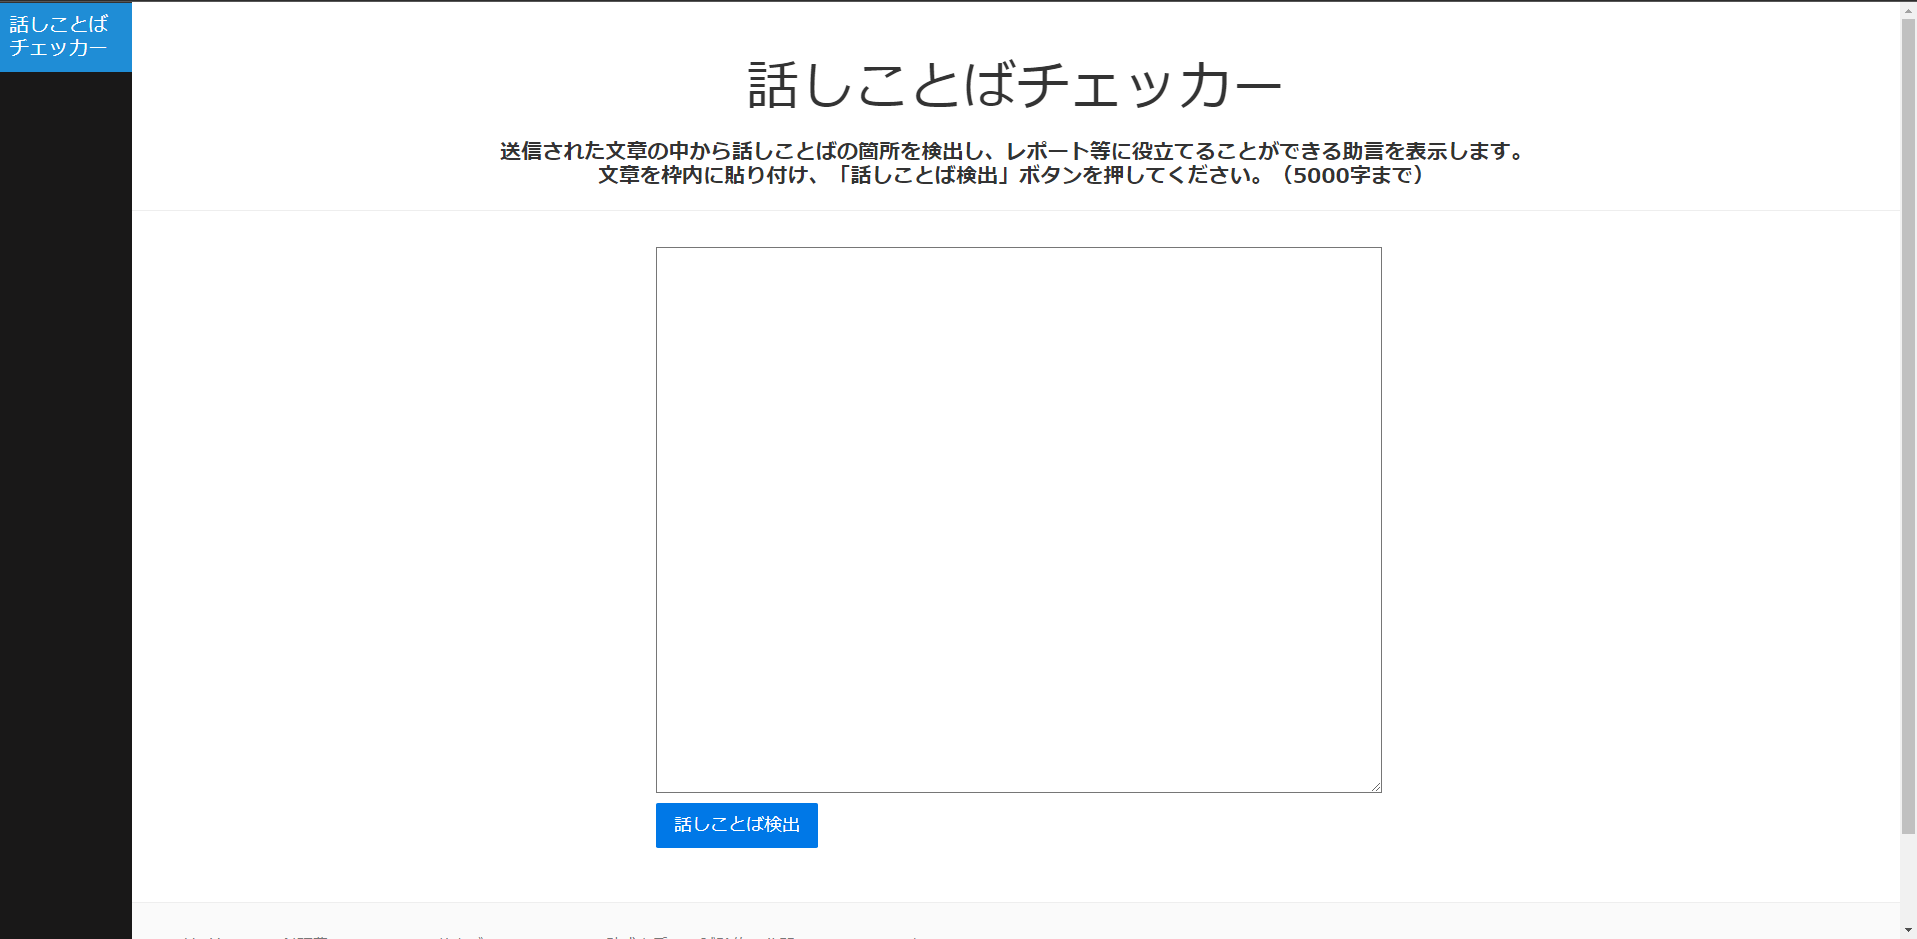
\includegraphics[width=150mm]{image/checkerss-plain.png}
	\caption{話しことばチェッカーの入力画面}
	\label{checkerss-plain}
\end{figure}

レポートなどの文章を入力し提出することで、文章中の話しことばの箇所が色付けされる。画面上で、色付けされた箇所にマウスを合わせると、書きことばへの修正例およびコメントといった推敲に役立つ情報が確認できる。実際の利用画面を図3.xに示す。

\begin{figure}[H]
	\centering
 	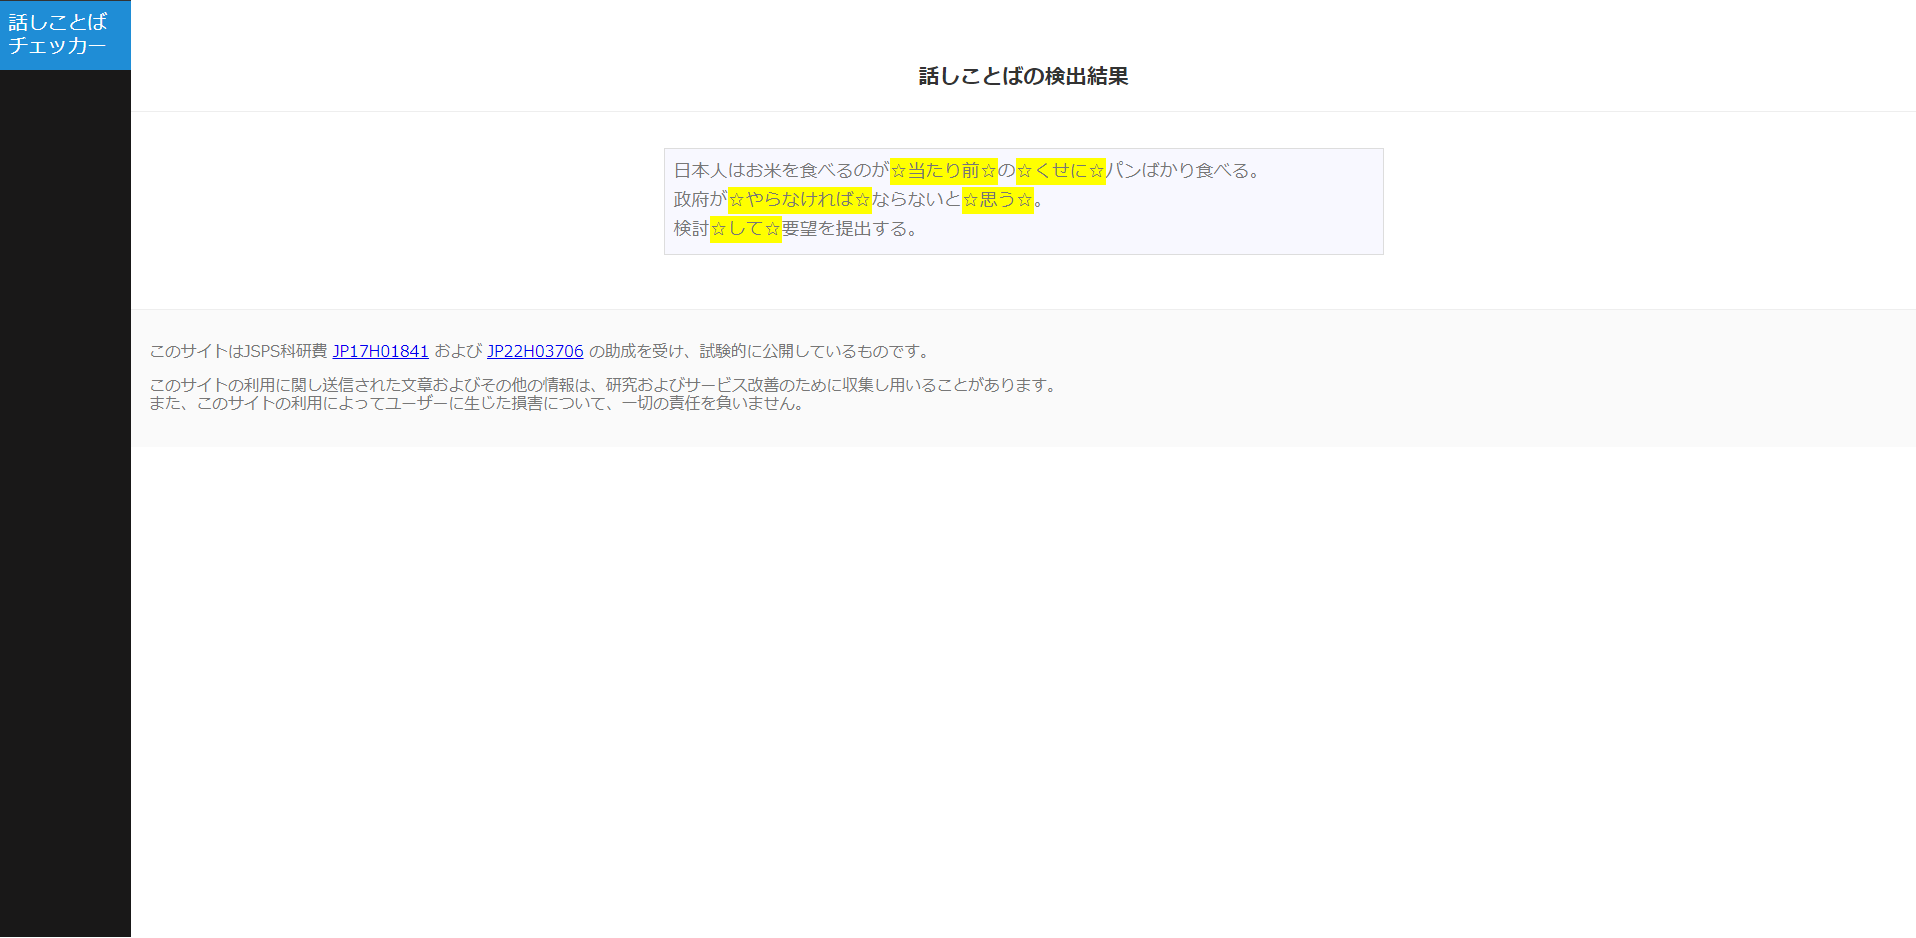
\includegraphics[width=150mm]{image/checkerss-result.png}
	\caption{話しことばチェッカーの話しことば検出画面}
	\label{checkerss-plain}
\end{figure}

\begin{figure}[H]
	\centering
 	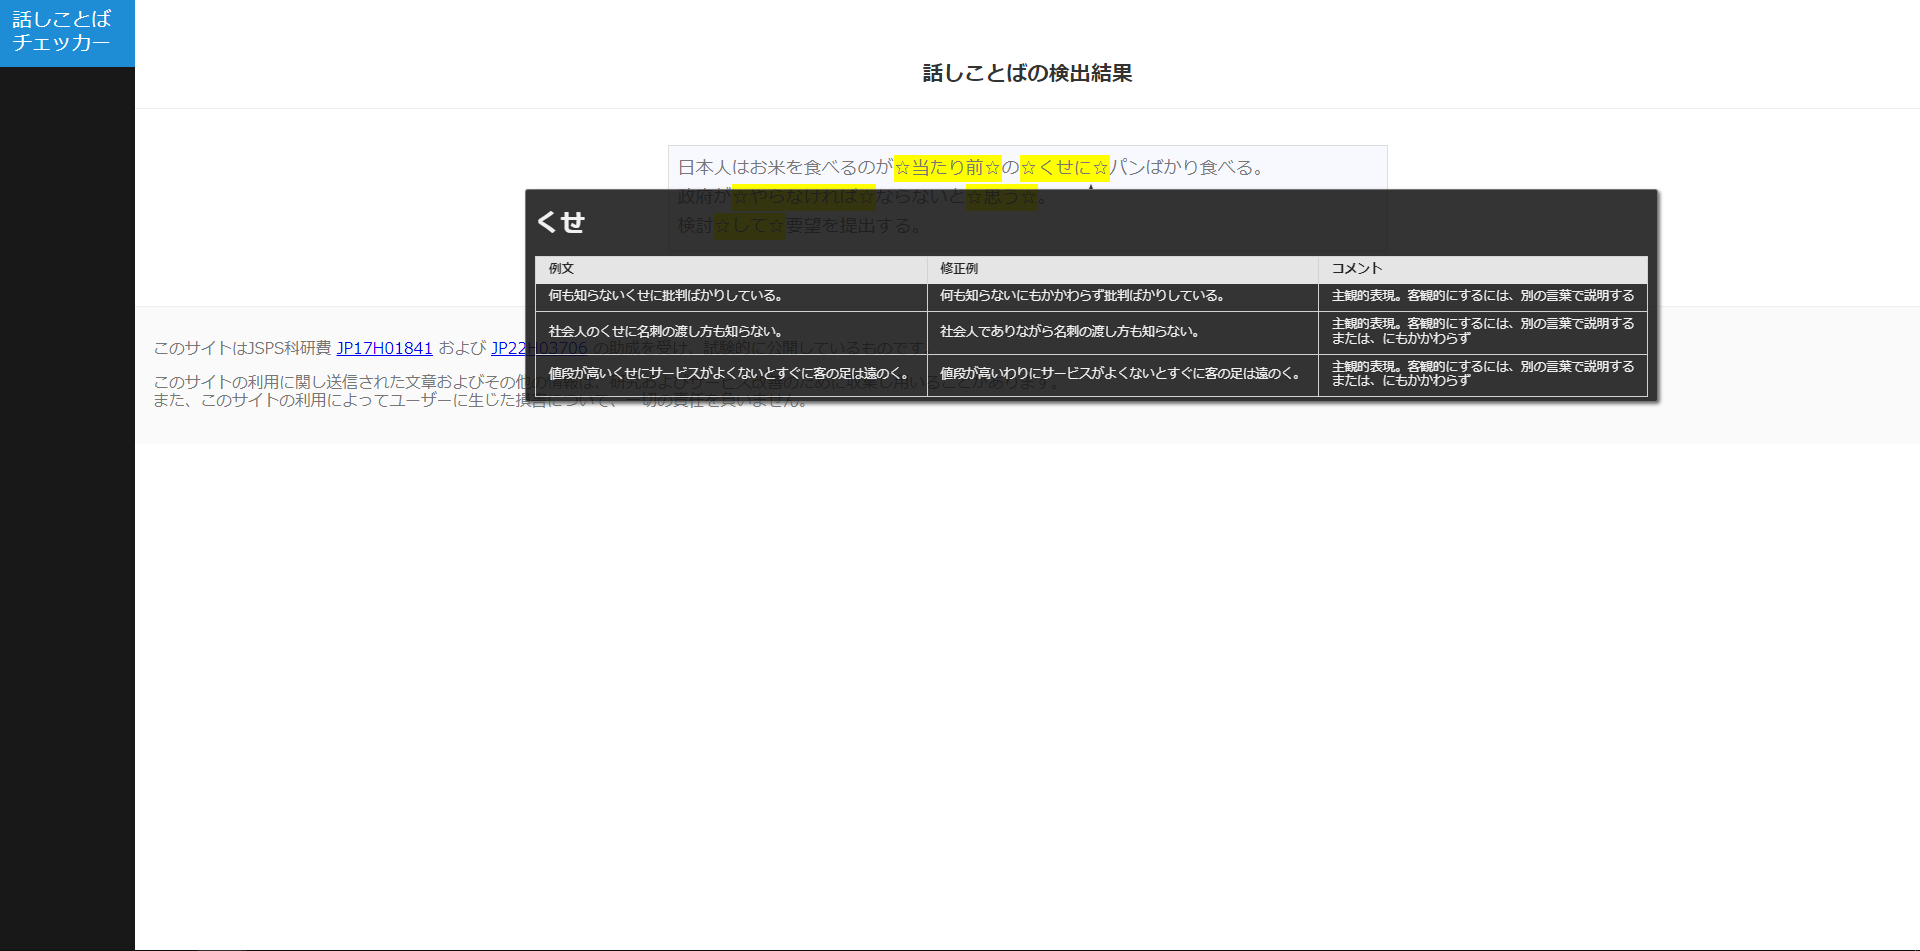
\includegraphics[width=150mm]{image/checkerss-popout.png}
	\caption{修正例などを表示している様子}
	\label{checkerss-plain}
\end{figure}



すべての話しことばのうち、INDEPENDENCE、PREFIX、SUFFIXに振り分けられている話しことばについては、現在運用している話しことばチェッカーで検出可である。一方で、COLLOCATION、OTHERに振り分けられえた話しことばは現状では不可能である。COLLOCATIONには、係り受けを伴う「~たり~たり」などの対象単語とそのほかに着目すべき単語との位置が離れているものがある。これは、話しことばの検出方式が対象単語とその前後に隣接する単語をチェックする仕様となっているためである。

現在使用されている話しことばデータベースは、話しことば事例集を基に設計されており、すべての話しことばが上記のカテゴリに分類することができる。しかし、本研究チームのこれまでの研究において、話しことばであるか書きことばであるかが不明瞭な表現が存在することがわかっており、これらの表現はカテゴリ分類を基にして話しことば検出を行っている本システムでは検出が困難である。本研究チームではこのような表現をグレーゾーンと定義している。

\section{話しことばにおけるグレーゾーン}
レポートに含まれる表現の中には、話しことばであるか書きことばであるかが不明瞭な表現が存在する。

\begin{table}[H]
\centering
\caption{グレーゾーンの例}
\begin{tabular}{|l|l|}
\hline
\multicolumn{1}{|c|}{表現} & \multicolumn{1}{c|}{例文} \\ \hline
てしまう   & \begin{tabular}[l]{@{}l@{}}アップライトピアノだと弾いている指が隠れてしまう\end{tabular} \\ \hline
残念      & \begin{tabular}[l]{@{}l@{}}楽しみにしていたイベントが中止になり残念だった\end{tabular} \\ \hline
面倒くさい & \begin{tabular}[l]{@{}l@{}}私生活では話すことを面倒くさがらずに、\\聞かれたことを真摯に答え説明する力をつけるように努力する\end{tabular} \\ \hline
厳しい     & \begin{tabular}[l]{@{}l@{}}ノルマを達成しなければ昇進は厳しい\end{tabular} \\ \hline
感じる     & \begin{tabular}[l]{@{}l@{}}人それぞれ大丈夫と感じることは異なっている\end{tabular} \\ \hline
大切      & \begin{tabular}[l]{@{}l@{}}社会で活躍できる人材を育成することも大切であると考える\end{tabular} \\ \hline
つらい     & \begin{tabular}[l]{@{}l@{}}芸能界は華やかに見えても、肉体的にも精神的にもつらい仕事がある\end{tabular} \\ \hline
\end{tabular}
\label{ambiguous-ex}
\end{table}

 % 
\chapter{第4章予定地\label{c4}}
\begin{comment}
機械学習
評価指標
など
\end{comment}

\section{4.1\label{c4s1}}
機会学習は、特定のタスクを効率的に処理するため、あるデータが持っているルールやパターンを反復学習を用いて学習し、そこから得られたパターンをもとに予測を行う技術である。2010年代にニューラルネットワークや自然言語処理が登場し、機械学習が再び注目されるようになった。
さらに、ハードウェアの性能の向上およびインターネットの発展により、機械学習に利用できる学習データを容易に収集できるようになったことから、ニューラルネットワークを用いた機械学習が広く用いられるようになった。ニューラルネットワークは、人体の脳の神経細胞であるニューロンおよびそのつながりである神経回路を数理モデルで表現したものである。
ニューラルネットワークが登場する前の機械学習では、データの特徴量などは人間の手によって設定されていたが、特徴量の調整などの調整は機械が自動で行うため、元のデータを与えることで、従来の人間の手による調整よりも高い精度で予測を行うことができる。

機械学習の分野の1つに自然言語処理がある.自然言語とは人間が日常的に使用している言語を指し,これをコンピュータを用いて処理する技術のことである.自然言語処理には大きく4つの段階でテキストデータの処理を行う.

\begin{enumerate}
    \item 形態素解析
    \item 構文解析
    \item 意味解析
    \item 文脈解析
\end{enumerate}

自然言語処理を行う上で,処理の対象となる文書データと,文書に含まれる単語を識別するための辞書が必要となる.自然言語処理分野において課題に挙げられることは,自然言語が本質的に持つ「曖昧さ」が挙げられ,これが文章の解釈が複雑になる要因となっている.これは,単語が持つ意味が複数存在し,その単語が用いられている文章の文脈によって意味が変化するためである.この影響を軽減させるためには,自然言語処理を行うモデルに大量のテキストデータを学習させる必要がある.

\section{二値分類における評価指標 \label{c4s2}}

\subsection{混合行列 \label{c4s2-1}}
機械学習における二値分類の評価指標に,混合行列(Confusion Matrix)がある.二値分類で出力されたクラス分類結果をまとめた行列であり,二値分類タスクを行う機械学習モデルの評価指標として利用される.
 
% 図挿入予定

混合行列左上のTP(True Positive)は,実際のデータが正であるものに対し正と予想されたデータの数である.FP(False Positive)は,実際のデータが正であるものに対し負と予想されたデータである.TN(True Negative)は,実際のデータが負であるものに対し負と予想されたデータである.FN(False Negative)は,実際のデータが負であるものに対し正と予想されたデータの個数である.これら4つの値を用いて,後述する正解率,再現率,適合率,F1値を算出する.

\subsubsection{正解率 \label{c4s2-1a}}
正解率(Accuracy)は,二値分類タスクの評価指標の一つであり,全体の分類結果のうち正答した割合を示す値である.正解率の定義を次式に示す.

$$
Accuracy = \frac{TP+FN}{TP+TN+FP+FN}
$$


\subsubsection{適合率 \label{c4s2-1b}}
適合率は(Precision)は,二値分類タスクにおける評価指標の一つであり,学習モデルが正と予測したもののうち,実際に正であものの割合を示す値である.適合率の定義を次式に示す.

$$
Precision = \frac{TP}{TP+FP}
$$


\subsubsection{再現率 \label{c4s2-1c}}
再現率(Recall)は,二値分類タスクの評価指標の一つれあり,実際のデータに含まれる正クラス全体のうち,学習モデルが正と予測したものの割合を示す値である.再現率の定義を次式に示す.

$$
Recall = \frac{TP}{TP+FN}
$$

\subsubsection{F1値 (F1-score, F-measure) \label{c4s2-1d}}
F1値は,二値分類タスクの一つであり,適合率と再現率の調和平均で算出される値である.適合率と再現率の関係はトレードオフの関係であるため,適合率と再現率の間に差が生じる場合がある.この場合,精度が良いとは一概には判断できない.そのため,これら2つの調和平均を算出し,精度に対し2値のバランスを判断するために用いられる.

$$
F1 = \frac{2 \times Recall \times Precision}{Recall+Precision}
$$


\section{Attention \label{c4s3}}
Attentionは、

\section{Transformer \label{c4s4}}
Transformer とは,再帰型ニューラルネットワーク (以下,RNN) を一切使わずに Attention のみを使うことで,入力と出力の文章同士の広範囲な依存関係を捉えられるモデルである.[7]
RNN は,単語が連続し順序が重要となるような時系列情報を扱うのに最適であるが,逐次的に処理を行うため,処理に多くの時間を必要とする.
また,離れた位置にある文,単語の依存関係をとらえることが難しいといった問題がある.
Transformerは以上のような問題点を克服したモデルである.
Transformerの構造を図aaaに示す.

\begin{figure}[H]%3.3
	\centering
	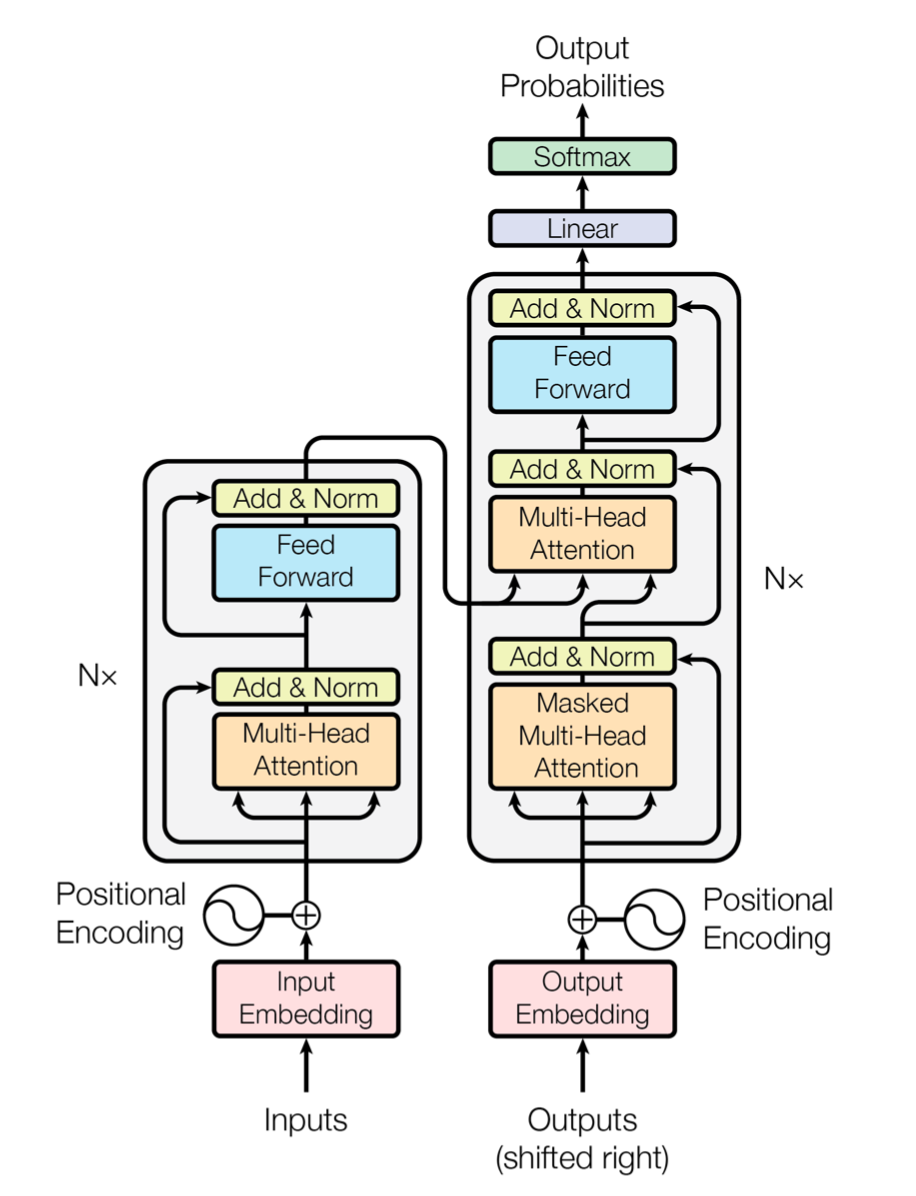
\includegraphics[width=120mm]{image/transformer.png}
	\caption{Transformerの構造}
	\label{transformer}
\end{figure}

\section{BERT \label{c4s5}}
\subsection{概要}
BERT とは,Bidirectional Encoder Representations from Transformers の略で, 「Transformerによる双方向のエンコード表現」と訳され,2018 年 10 月に Google の Jacob Devlin らの論文[6] で発表された自然言語処理モデルである.
また,質問応答 (Question Answering) や自然言語推論 (Multi Natural Language Inference) などの 11 種の自然言語処理タスクにおいて当時の最高性能を達成している手法であり,これ以降,このモデルから派生して作られたモデルが多数存在する.
また,現在の Google の検索エンジンにも用いられている.
BERT の学習は,大きく2段階に分けられる.
1つ目がラベル付けされていないデータを学習させる「事前学習」であり,2つ目が事前学習時と比較的少量のデータを用いる「Fine Tuning」である.
事前学習で汎用的なモデルを作成し,Fine Tuningを行うことで,個々のタスクに適応したモデルを作成する.

\subsection{アーキテクチャ}
BERTのモデルアーキテクチャは,双方向のtransformerのエンコーダとなっている.
図aaaにBERTと,BERTと同様に事前学習を利用する自然言語処理モデルを比較したものを示す.

% %\begin{figure}[H]
% 	\centering
% % 	\includegraphics[width=150mm]{image/architechture.png}
% 	\caption{各モデルの構造}
% 	\label{architechture}
% \end{figure}

% \subsubsection{Transformers}
% Transformer とは,再帰型ニューラルネットワーク (以下,RNN) を一切使わずに Attention のみを使うことで,入力と出力の文章同士の広範囲な依存関係を捉えられるモデルである.[7]
% RNN は,単語が連続し順序が重要となるような時系列情報を扱うのに最適であるが,逐次的に処理を行うため,処理に多くの時間を必要とする.
% また,離れた位置にある文,単語の依存関係をとらえることが難しいといった問題がある.
% Transformerは以上のような問題点を克服したモデルである.
% Transformerの構造を図aaaに示す.

% \begin{figure}[H]%3.3
% 	\centering
% 	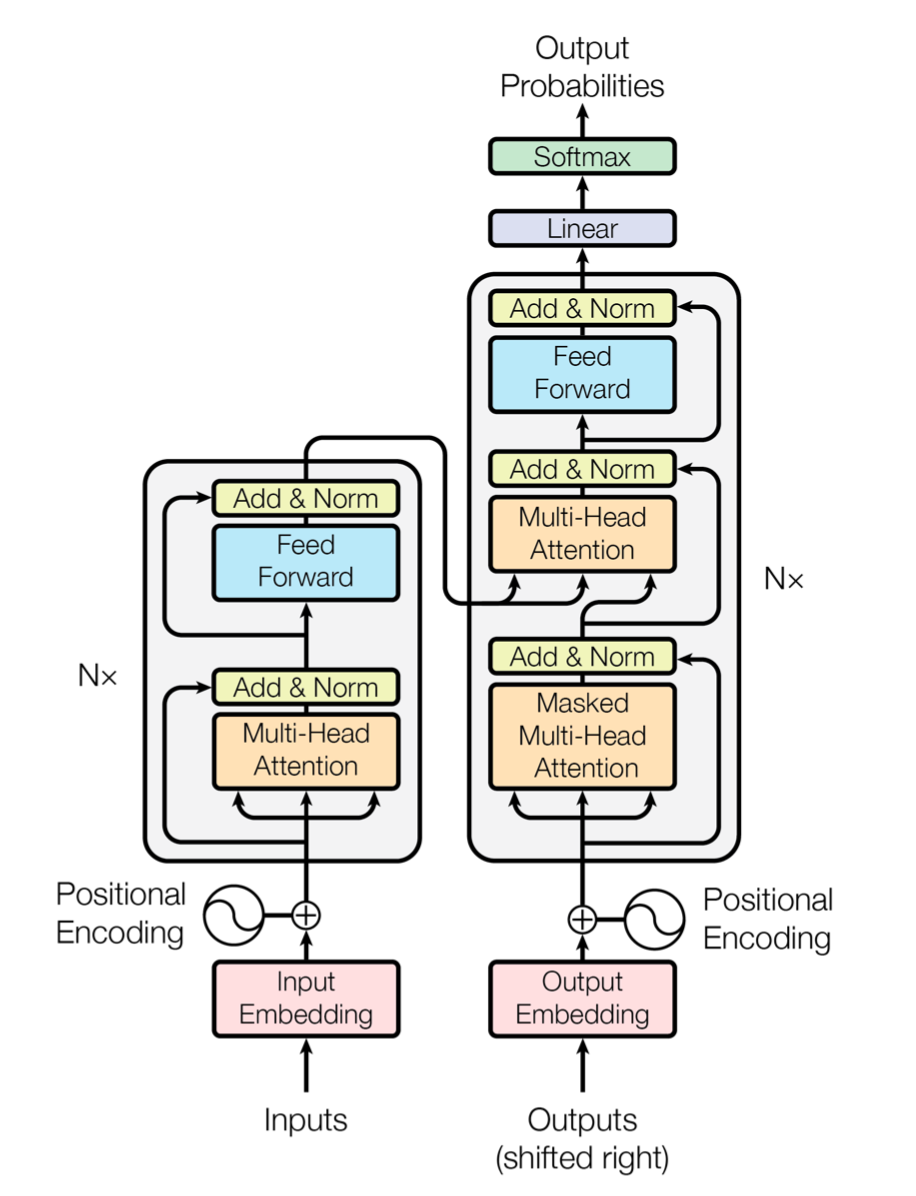
\includegraphics[width=100mm]{image/transformer.png}
% 	\caption{Transformerの構造}
% 	\label{transformer}
% \end{figure}

\subsubsection{Attention}
Attention とは,先述の通り,Transformer の中枢を担う仕組みである.
自然言語処理においては,単語の意味を理解するために,文中のどの単語に注目するすべきかを示すスコアである.Query:${Q}$,Key:${K}$,Value:${V}$の3つのベクトルから計算される.
${K}$と${V}$は1対1の組である.
Attentionは,Self-AttentionとSource-Target-Attentionの2種類がある.また,Attentionの算出方法は加法を使う場合と内積を使う場合があるが,Transformerで使うAttentionは内積を使って算出するため,以降のAttentionの計算は内積を使用していることを前提とする.

\begin{itemize}
	\item Self-Attention \par
	${Q}$, ${K}$, ${V}$は全て同じデータから得られた値を使用する.
	例として「私/は/大学生/です」という文から${Q}$を得たとすると,${K}$, ${V}$も同じ文から取得する.Transformer では Encoder, Decoder の両方に採用され,文の構造や,形態素同士の関係(例文では「私」=「大学生」)を獲得するために使用される.

	\item Target-Attention \par
	${Q}$と${K}$, ${V}$は異なるデータから得られた値を使用する(${K}$, ${V}$は同じデータから取得する).
	例として「風邪/を/引いた」,「病院/に/行く」という2文があるとき,${Q}$は「風邪/を/引いた」から,${K}$, ${V}$は「病院/に/行く」から取得する.
	 Transfomer では Decoder で採用され,「風邪/を/引いた」→「病院/に/行く」という対話の学習に用いられる.
	入力文に対応する出力文が出力されるように学習を行う.
\end{itemize}

以上の Attention を基本とし,Transformers では Scaled Dot-Product Attention と Multi-Head Attentionが実装されている.
その仕組みを図aaa,図aaaに示す.

% % \begin{figure}[H]
% 	\centering
% 	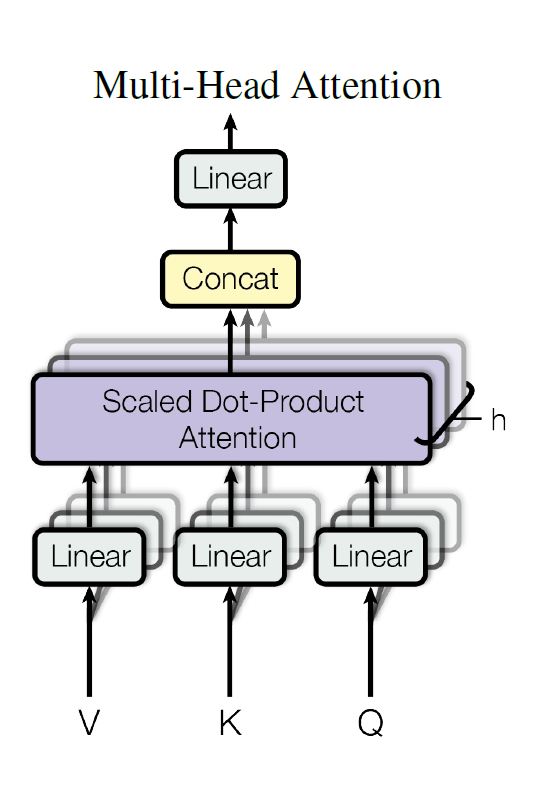
\includegraphics[width=80mm]{image/transformer-multi-head-attention.png}
% 	\caption{Multi-Head Attentionの構造}
% 	\label{mha}
% \end{figure}

% % \begin{figure}[H]
% 	\centering
% 	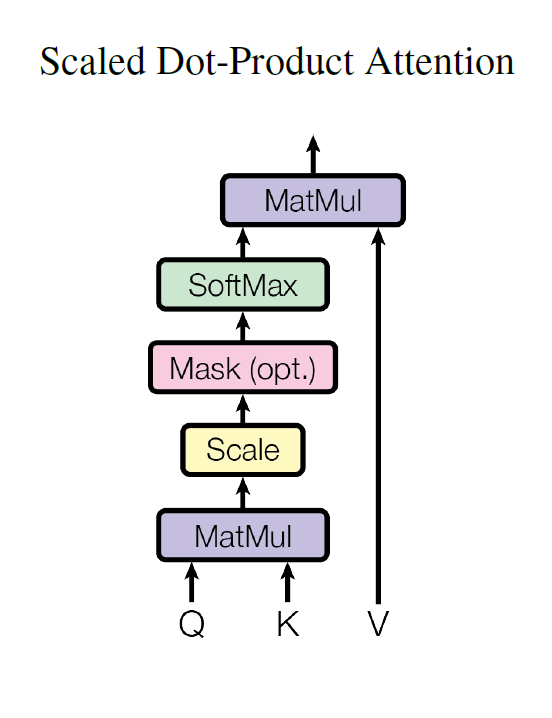
\includegraphics[width=80mm]{image/transformer-scaled-dot-product-attention.png}
% 	\caption{Scaled Dot-Product Attentionの構造}
% 	\label{sda}
% \end{figure}

% 	${Q}$ ${K}$ ${V}$

\begin{itemize}
\item Scaled Dot-Product Attention \par
\par ${Q}$に対応する${K}$を探し,その${K}$を元にして対応する${V}$を取得する.
まず,${Q}$と${K}$の内積${QK^T}$を取ることで${Q}$に対する${K}$の関連度を算出する.
次に softmax 関数を用いて正規化する.ここで,正規化された値は,Attention の重みであり${Q}$に対応する${K}$の位置を示している.
次に Attention の重みと${V}$の内積を求め,${K}$の位置に対応する${V}$を加重和として取得する.
図 3.5 の数式を式(\ref{attention})に,softmax 関数を式(\ref{softmax})に示す.

\begin{equation}
    \mbox{Attention}(Q,K,V) = \mbox{softmax}\left( \frac{QK^T}{\sqrt{d_k}}\right)
    \label{attention}
\end{equation}

\begin{equation}
    \label{softmax}
    \frac{\exp(a_i)}{\sum_{j=1}^{n}\exp(a_j)} \quad(i=1,...,n)
\end{equation}

${QK^T}$の値は次元数に比例して大きくなり,勾配は小さくなってしまう.
そこで式\ref{attention}では${QK^T}$を${\sqrt{d_k}}$で割ることで${QK^T}$の値の増大を防いでいる.
ここで,${d_k}$は${Q}$の次元数を後述する Multi-Head Attention の Head 数で割った値である.

\begin{equation}
    \label{dk}
    d_k = \frac{Q\mbox{の次元数}}{\mbox{Multi-Head Attention のHead数}}
\end{equation}

\item Multi-Head Attention \par
Multi-Head Attention は,Scaled Dot-Product Attention を1つの Head として,複数の Head を並列で処理する仕組みである.
仮に,Head 数が 8 , ${Q}$, ${K}$, ${V}$ の次元数が 512 とすると${\frac{512}{8}=64}$であり,次元数が 64 の ${Q}$, ${K}$, ${V}$ を用いた Scaled Dot-Product Attention を並列に 8 個処理することになる.最終的には個別に計算された値を 1 つのベクトルに落とし込む(concat)ことで単語の分散表現を得る.
この Multi-Head Attention を 1 つのユニット(図 3.2 の Trm )として全結合的に接続したものが BERT モデルである.

\end{itemize}

\section{LLM \label{c4s6}}
LLMとは、Large Language Model の略称であり、大規模言語モデルと呼ばれる。大規模言語モデルという用語についての正式な定義はないが、大規模コーパスを用いて事前学習を行っており、パラメータ総数が数百万以上の言語モデルを指して言われることが多い。LLMの例として、先述のBERTやOpenAI社が開発したGPT-3が挙げられる。

 % 機械学習
\chapter{第5章予定地[検証?] \label{c5}}

\section{5.1 \label{c5s1}}
話しことばチェッカーの現状の課題
グレーゾーンの検出ができていない
機械学習は有効であることが示唆されている。
課題点は事例収集

現在運用している話しことばチェッカーの



\section{5.2 \label{c5s2}}

\begin{table}[H]
\centering
\caption{あああ}
\begin{tabular}{|r|}
\hline
\multicolumn{1}{|c|}{カテゴリ} \\ \hline
\begin{tabular}[r]{@{}r@{}}0.00 \end{tabular} \\ \hline
\begin{tabular}[r]{@{}r@{}}0.00 \end{tabular}  \\ \hline
\begin{tabular}[r]{@{}r@{}}0.00 \end{tabular}  \\ \hline
\begin{tabular}[r]{@{}r@{}}0.00 \end{tabular}  \\ \hline
\end{tabular}
\label{spoken-book}
\end{table} % 検証?
\chapter{LLMを用いた話しことば検出}

\begin{comment}
書きことばリストは、話しことばチェッカーで検出しない表現をもとに選んでいる。
それでもchatGPTが出力する場合は、チェッカーの癖もあり得る。← これは要相談
\end{comment} % 
\clearpage
\addcontentsline{toc}{chapter}{参考文献} %章立てせずに目次に追加するおまじない
\renewcommand{\bibname}{参考文献} %これがないと,タイトルが「関連図書」になってしまう
\begin{thebibliography}{99999}
\bibitem{checker}
学生のレポートにおける話し言葉とその出現傾向,日本語日本文学 第 28 号 p57-p71, 
山下由美子,2018



\end{thebibliography}

% \chapter*{謝辞}

本研究を行うにあたり、主査としてご指導及びご鞭撻をいただきました、公立千歳科学技術大学 小松川 浩 教授に心より感謝申し上げます。学部4年次から3年の間、至らぬ点も多く、多大な迷惑をかけました。% 無事に論文を書き上げることができました。重ねて御礼申し上げます。
副査の公立千歳科学技術大学 萩原 茂樹 教授

\begin{comment}
label命名規則
1. c[n] : 第n章のラベル
2. c[m]s[n] : 第m章第n節のラベル
\end{comment}


\end{document}